\documentclass[border=3pt]{standalone}
% Preâmbulo compartilhado pelos diagramas TikZ da aula 8 de IHR (Métodos de Pesquisa)
\usepackage[T1]{fontenc}
\usepackage[utf8]{inputenc}
\usepackage{lmodern}
\usepackage{amsmath}
\usepackage{xcolor}
\usepackage{tikz}
\usetikzlibrary{arrows.meta,angles,quotes,decorations.pathmorphing,decorations.pathreplacing,calc,
                positioning,shapes.geometric,shapes.misc,backgrounds,fit,
                math}

% Paleta (mesma dos SVGs originais)
% Paleta da disciplina de IHR: acento azul (#1A6FB5), cor de destaque do tema.
% (o nome "dblue" é mantido para não alterar todos os diagramas)
\definecolor{dblue}{HTML}{1A6FB5}
\definecolor{dorange}{HTML}{B3541E}
\definecolor{dgreen}{HTML}{4A7C59}
\definecolor{dred}{HTML}{9C4B4B}
\definecolor{dcream}{HTML}{F4F1EA}
\definecolor{dshade}{HTML}{DDD7C9}

% Função gaussiana (não normalizada por padrão de escala visual)
\pgfmathdeclarefunction{gauss}{3}{%
  \pgfmathparse{1/(#3*sqrt(2*pi))*exp(-((#1-#2)^2)/(2*#3^2))}%
}

% Estilos comuns (prefixo d... para não colidir com chaves internas do pgf)
\tikzset{
  >={Stealth[length=2mm]},
  dguide/.style={gray!55, dashed, line width=0.4pt},
  daxis/.style={gray!60, line width=0.7pt, ->},
  dbody/.style={fill=black!3, draw=black!80, line width=1pt},
  dacc/.style={draw=dblue, line width=1pt},
  dlbl/.style={black!55, font=\small},
  dsub/.style={black!45, font=\footnotesize},
  dstate/.style={circle, draw=black!80, fill=dcream, line width=1pt,
                 minimum size=17mm, font=\large, inner sep=1pt},
  dobs/.style={circle, draw=black!80, fill=dshade, line width=1pt,
               minimum size=14mm, font=\large, inner sep=1pt},
  dbox/.style={rounded corners=2pt, draw=black!80, fill=dcream, line width=1pt,
               align=center, inner sep=6pt},
  dop/.style={circle, draw=black!80, fill=white, line width=1pt,
              minimum size=6mm, inner sep=0pt, font=\small},
  dtrans/.style={->, dblue, line width=1pt},
  dmeas/.style={->, dorange, line width=1pt},
  dcurve/.style={line width=1pt, dblue},
  dcurveb/.style={line width=1.4pt, dorange},
}

\begin{document}
\hyphenpenalty=10000 \exhyphenpenalty=10000 \tolerance=9999 \emergencystretch=3em
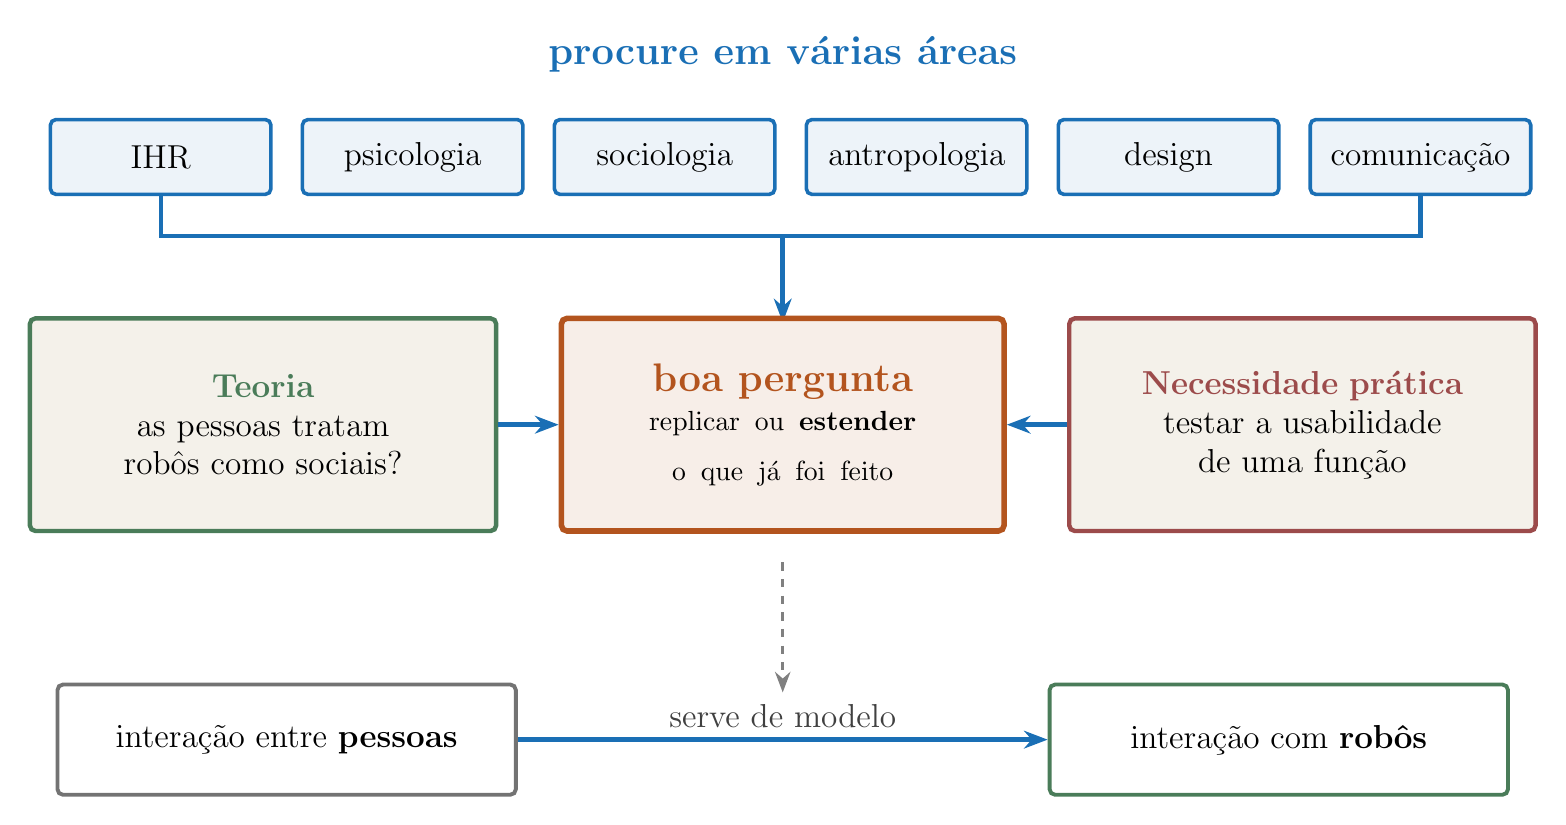
\begin{tikzpicture}[x=1cm,y=1cm]
  \tikzset{chip/.style={dbox, draw=dblue, fill=dblue!8, line width=1.3pt, minimum width=2.8cm, minimum height=0.95cm, font=\large},
           card/.style={dbox, text width=5.5cm, minimum height=2.7cm, font=\large, line width=1.6pt, align=center}}
  % ---------- onde procurar ----------
  \node[font=\Large\bfseries, dblue] at (9.6,9.3) {procure em várias áreas};
  \node[chip] at (1.7,8.0) {IHR};
  \node[chip] at (4.9,8.0) {psicologia};
  \node[chip] at (8.1,8.0) {sociologia};
  \node[chip] at (11.3,8.0) {antropologia};
  \node[chip] at (14.5,8.0) {design};
  \node[chip] at (17.7,8.0) {comunicação};
  \draw[dblue, line width=1.5pt] (1.7,7.5) -- (1.7,7.0) -- (17.7,7.0) -- (17.7,7.5);
  \draw[dtrans, line width=1.8pt, -{Stealth[length=3mm]}] (9.6,7.0) -- (9.6,5.9);
  % ---------- origens da pergunta ----------
  \node[card, draw=dgreen] (t) at (3.0,4.6) {\textbf{\textcolor{dgreen}{Teoria}}\\ as pessoas tratam\\ robôs como sociais?};
  \node[card, draw=dred] (n) at (16.2,4.6) {\textbf{\textcolor{dred}{Necessidade prática}}\\ testar a usabilidade\\ de uma função};
  \node[dbox, draw=dorange, fill=dorange!10, line width=2pt, text width=5.2cm, minimum height=2.7cm, font=\Large\bfseries, align=center] (q) at (9.6,4.6) {\textcolor{dorange}{boa pergunta}\\[2pt] {\normalsize\mdseries replicar ou \textbf{estender}\\ o que já foi feito}};
  \draw[dtrans, line width=1.8pt, -{Stealth[length=3mm]}] (t.east) -- (q.west);
  \draw[dtrans, line width=1.8pt, -{Stealth[length=3mm]}] (n.west) -- (q.east);
  % ---------- modelo: interação entre pessoas ----------
  \node[dbox, draw=black!55, fill=white, line width=1.4pt, text width=5.4cm, minimum height=1.4cm, font=\large, align=center] (p) at (3.3,0.6) {interação entre \textbf{pessoas}};
  \node[dbox, draw=dgreen, fill=white, line width=1.4pt, text width=5.4cm, minimum height=1.4cm, font=\large, align=center] (r) at (15.9,0.6) {interação com \textbf{robôs}};
  \draw[dtrans, line width=1.8pt, -{Stealth[length=3mm]}] (p.east) -- node[above, font=\large, black!75] {serve de modelo} (r.west);
  \draw[black!50, dashed, line width=1.2pt, -{Stealth[length=2.6mm]}] (9.6,2.85) -- (9.6,1.2);
\end{tikzpicture}
\end{document}
